\documentclass[10pt,a4paper]{article}

% content/resources/templates/preamble.tex
\usepackage[margin=0.6in]{geometry}
\author{Milav Dabgar}
\usepackage{amsmath,amssymb,amsthm}
\usepackage{booktabs}
\usepackage{multirow}
\usepackage{xcolor}
\usepackage{tcolorbox}
\tcbuselibrary{breakable,skins}
\usepackage[colorlinks=true,linkcolor=blue]{hyperref}
\usepackage{titlesec}
\usepackage{enumitem}
\usepackage{tikz}
\usepackage{pgfplots}
\usepackage{circuitikz}
\usepackage[version=4]{mhchem}
\usepackage{longtable}
\usepackage{array}
\usepackage{float}
\usepackage{caption}
\usepackage{listings}

\lstset{
  basicstyle=\small\ttfamily,
  breaklines=true,
  breakatwhitespace=false,
  postbreak=\mbox{\textcolor{red}{$\hookrightarrow$}\space},
  float=false,
  numbers=left,
  numberstyle=\tiny\color{gray},
  numbersep=10pt,
  xleftmargin=2em,
  keywordstyle=\color{blue},
  commentstyle=\color{green!60!black},
  stringstyle=\color{purple},
  backgroundcolor=\color{gray!5},
  showstringspaces=false,
  tabsize=2,
  captionpos=b,
  keepspaces=true,
  columns=flexible
}

\pgfplotsset{compat=1.18}
\usetikzlibrary{shapes,arrows,positioning,calc,patterns,decorations.pathmorphing,decorations.markings,arrows.meta}

% Color scheme
\definecolor{headcolor}{RGB}{0,102,204}
\definecolor{keycolor}{RGB}{220,20,60}
\definecolor{solutioncolor}{RGB}{34,139,34}
\definecolor{mnemoniccolor}{RGB}{148,0,211}
\definecolor{codecolor}{RGB}{0,0,100}

% Spacing
\setlength{\parskip}{3pt}
\setlist[itemize]{nosep}
\setlist[enumerate]{nosep}

% Title formatting
\titleformat{\section}{\Large\bfseries\color{headcolor}}{\thesection}{1em}{}
\titleformat{\subsection}{\large\bfseries\color{headcolor}}{\thesubsection}{1em}{}

% Pandoc tightlist compatibility
\providecommand{\tightlist}{%
  \setlength{\itemsep}{0pt}\setlength{\parskip}{0pt}}

% Pandoc longtable compatibility
\newcounter{none}
\def\thenone{}


% content/resources/templates/english-boxes.tex
% This file is currently empty - it exists to maintain consistency with the import structure.
% Add custom environments here if needed in the future.


\begin{document}

\begin{center}
{\Huge\bfseries\color{headcolor} Mathematics-I Solutions}\\[5pt]
{\LARGE DI01000021 -- Summer 2025}\\[3pt]
{\large Semester 1 Study Material}\\[3pt]
{\normalsize\textit{Detailed Solutions and Explanations}}
\end{center}

\vspace{10pt}

\section*{Question 1 [14 marks]}

\textbf{Fill in the blanks/MCQs using appropriate choice from the given options}

\subsection*{Q1.1 [1 mark]}
\textbf{$\log_3 1 = $ \_\_\_\_\_\_\_}

\begin{solutionbox}
\textbf{Answer}: d. 0

\textbf{Solution}:
For any base $a > 0, a \neq 1$: $\log_a 1 = 0$
Therefore: $\log_3 1 = 0$
\end{solutionbox}

\subsection*{Q1.2 [1 mark]}
\textbf{The modulus of the complex number $z = 3 + 4i$ is \_\_\_\_\_\_\_}

\begin{solutionbox}
\textbf{Answer}: a. 5

\textbf{Solution}:
$|z| = \sqrt{a^2 + b^2} = \sqrt{3^2 + 4^2} = \sqrt{9 + 16} = \sqrt{25} = 5$
\end{solutionbox}

\subsection*{Q1.3 [1 mark]}
\textbf{The value of $\lim_{x \to 0} \frac{\tan x}{x}$ is \_\_\_\_\_\_\_}

\begin{solutionbox}
\textbf{Answer}: b. 1

\textbf{Solution}:
Standard limit identity.
\end{solutionbox}

\subsection*{Q1.4 [1 mark]}
\textbf{If $A = \begin{bmatrix} 2 & 3 \\ 1 & 0 \end{bmatrix}$, then $|A| = $ \_\_\_\_\_\_\_}

\begin{solutionbox}
\textbf{Answer}: c. -3

\textbf{Solution}:
$|A| = (2)(0) - (3)(1) = 0 - 3 = -3$
\end{solutionbox}

\subsection*{Q1.5 [1 mark]}
\textbf{The derivative of $\sin x$ is \_\_\_\_\_\_\_}

\begin{solutionbox}
\textbf{Answer}: a. $\cos x$

\textbf{Solution}:
Standard differentiation formula.
\end{solutionbox}

\subsection*{Q1.6 [1 mark]}
\textbf{$\int_0^1 x dx = $ \_\_\_\_\_\_\_}

\begin{solutionbox}
\textbf{Answer}: b. 1/2

\textbf{Solution}:
$\int x dx = x^2/2$.
Value = $[\frac{1^2}{2}] - [\frac{0^2}{2}] = 1/2 - 0 = 0.5$
\end{solutionbox}

\subsection*{Q1.7 [1 mark]}
\textbf{If two lines slopes $m_1$ and $m_2$ are perpendicular, then \_\_\_\_\_\_\_}

\begin{solutionbox}
\textbf{Answer}: c. $m_1 m_2 = -1$

\textbf{Solution}:
Condition for perpendicularity of two lines.
\end{solutionbox}

\subsection*{Q1.8 [1 mark]}
\textbf{The value of $i^{4}$ is \_\_\_\_\_\_\_}

\begin{solutionbox}
\textbf{Answer}: a. 1

\textbf{Solution}:
$i^2 = -1$.
$i^4 = (i^2)^2 = (-1)^2 = 1$.
\end{solutionbox}

\subsection*{Q1.9 [1 mark]}
\textbf{The conjugate of $2 - 3i$ is \_\_\_\_\_\_\_}

\begin{solutionbox}
\textbf{Answer}: b. $2 + 3i$

\textbf{Solution}:
To find conjugate, change sign of imaginary part.
\end{solutionbox}

\subsection*{Q1.10 [1 mark]}
\textbf{The radius of the circle $x^2 + y^2 = 36$ is \_\_\_\_\_\_\_}

\begin{solutionbox}
\textbf{Answer}: d. 6

\textbf{Solution}:
Standard form $x^2 + y^2 = r^2$.
$r^2 = 36 \Rightarrow r = 6$
\end{solutionbox}

\subsection*{Q1.11 [1 mark]}
\textbf{If vectors $\vec{a}$ and $\vec{b}$ are parallel, then \_\_\_\_\_\_\_}

\begin{solutionbox}
\textbf{Answer}: a. $\vec{a} \times \vec{b} = 0$

\textbf{Solution}:
Cross product of parallel vectors is zero vector.
\end{solutionbox}

\subsection*{Q1.12 [1 mark]}
\textbf{The dot product of $\vec{i}$ and $\vec{j}$ is \_\_\_\_\_\_\_}

\begin{solutionbox}
\textbf{Answer}: c. 0

\textbf{Solution}:
Orthogonal unit vectors have dot product zero.
\end{solutionbox}

\subsection*{Q1.13 [1 mark]}
\textbf{The degree of differential equation $\frac{d^2y}{dx^2} + (\frac{dy}{dx})^3 = 0$ is \_\_\_\_\_\_\_}

\begin{solutionbox}
\textbf{Answer}: a. 1

\textbf{Solution}:
Degree is the power of the highest order derivative.
Highest order derivative is $\frac{d^2y}{dx^2}$, its power is 1.
\end{solutionbox}

\subsection*{Q1.14 [1 mark]}
\textbf{The value of $\cos(0)$ is \_\_\_\_\_\_\_}

\begin{solutionbox}
\textbf{Answer}: b. 1

\textbf{Solution}:
Standard trigonometric value.
\end{solutionbox}

\section*{Question 2 [14 marks]}

\subsection*{Q2.a [3 marks]}
\textbf{Evaluate the determinant: $\begin{vmatrix} 1 & 2 & 3 \\ 4 & 5 & 6 \\ 7 & 8 & 9 \end{vmatrix}$}

\begin{solutionbox}
\textbf{Solution}:
$= 1(45 - 48) - 2(36 - 42) + 3(32 - 35)$
$= 1(-3) - 2(-6) + 3(-3)$
$= -3 + 12 - 9$
$= 12 - 12 = 0$
\end{solutionbox}

\subsection*{Q2.b [4 marks]}
\textbf{If $A = \begin{bmatrix} 1 & 2 \\ 3 & 4 \end{bmatrix}$ and $B = \begin{bmatrix} 5 & 6 \\ 7 & 8 \end{bmatrix}$, find $AB$.}

\begin{solutionbox}
\textbf{Solution}:
$AB = \begin{bmatrix} (1)(5)+(2)(7) & (1)(6)+(2)(8) \\ (3)(5)+(4)(7) & (3)(6)+(4)(8) \end{bmatrix}$
$AB = \begin{bmatrix} 5+14 & 6+16 \\ 15+28 & 18+32 \end{bmatrix}$
$AB = \begin{bmatrix} 19 & 22 \\ 43 & 50 \end{bmatrix}$
\end{solutionbox}

\subsection*{Q2.c [7 marks]}
\textbf{Graph of $\sin x$ vs $\cos x$ in $[0, \pi]$.}

\begin{solutionbox}
\textbf{Solution}:
Plot both functions on same axis.

\begin{center}
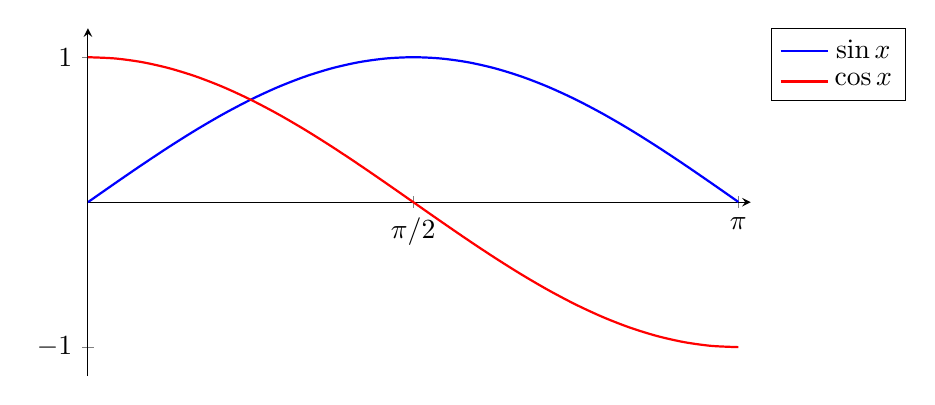
\begin{tikzpicture}
\begin{axis}[
    axis lines=middle,
    xmin=0, xmax=3.2,
    ymin=-1.2, ymax=1.2,
    xtick={0, 1.57, 3.14},
    xticklabels={$0$, $\pi/2$, $\pi$},
    ytick={-1, 1},
    legend pos=outer north east,
    width=10cm, height=6cm
]
\addplot[smooth, thick, blue, domain=0:3.14] {sin(deg(x))}; \addlegendentry{$\sin x$};
\addplot[smooth, thick, red, domain=0:3.14] {cos(deg(x))}; \addlegendentry{$\cos x$};
\end{axis}
\end{tikzpicture}
\end{center}
Intersection at $x=\pi/4$.
\end{solutionbox}

\section*{Question 3 [14 marks]}

\subsection*{Q3.a [3 marks]}
\textbf{Find complex conjugate and modulus of $z = \frac{3+4i}{1-2i}$.}

\begin{solutionbox}
\textbf{Solution}:
Rationalize denominator:
$z = \frac{(3+4i)(1+2i)}{(1-2i)(1+2i)} = \frac{3 + 6i + 4i + 8i^2}{1 - 4i^2}$
$z = \frac{3 + 10i - 8}{1 + 4} = \frac{-5 + 10i}{5} = -1 + 2i$

Conjugate $\bar{z} = -1 - 2i$
Modulus $|z| = \sqrt{(-1)^2 + 2^2} = \sqrt{1+4} = \sqrt{5}$
\end{solutionbox}

\subsection*{Q3.b [4 marks]}
\textbf{Find the angle between vectors $\vec{a} = i + j$ and $\vec{b} = i - j$.}

\begin{solutionbox}
\textbf{Solution}:
$\vec{a} \cdot \vec{b} = |\vec{a}| |\vec{b}| \cos \theta$
Dot product: $(1)(1) + (1)(-1) = 1 - 1 = 0$
Magnitudes: $|\vec{a}| = \sqrt{2}, |\vec{b}| = \sqrt{2}$

$0 = \sqrt{2}\sqrt{2} \cos \theta \Rightarrow \cos \theta = 0$
$\theta = 90^\circ$ or $\pi/2$ radians.
\end{solutionbox}

\subsection*{Q3.c [7 marks]}
\textbf{Verify Cayley-Hamilton Theorem for $A = \begin{bmatrix} 1 & 2 \\ 3 & 4 \end{bmatrix}$.}

\begin{solutionbox}
\textbf{Solution}:
Characteristic equation: $|A - \lambda I| = 0$
$\begin{vmatrix} 1-\lambda & 2 \\ 3 & 4-\lambda \end{vmatrix} = 0$
$(1-\lambda)(4-\lambda) - 6 = 0$
$4 - \lambda - 4\lambda + \lambda^2 - 6 = 0$
$\lambda^2 - 5\lambda - 2 = 0$

By theorem, $A$ satisfies this equation:
$A^2 - 5A - 2I = 0$

Calculate $A^2$:
$A^2 = \begin{bmatrix} 1 & 2 \\ 3 & 4 \end{bmatrix} \begin{bmatrix} 1 & 2 \\ 3 & 4 \end{bmatrix} = \begin{bmatrix} 7 & 10 \\ 15 & 22 \end{bmatrix}$

Substitute into equation:
$\begin{bmatrix} 7 & 10 \\ 15 & 22 \end{bmatrix} - 5\begin{bmatrix} 1 & 2 \\ 3 & 4 \end{bmatrix} - 2\begin{bmatrix} 1 & 0 \\ 0 & 1 \end{bmatrix}$
$= \begin{bmatrix} 7-5-2 & 10-10-0 \\ 15-15-0 & 22-20-2 \end{bmatrix} = \begin{bmatrix} 0 & 0 \\ 0 & 0 \end{bmatrix} = O$

Hence Verified.
\end{solutionbox}

\section*{Question 4 [14 marks]}

\subsection*{Q4.a [3 marks]}
\textbf{Differentiate $y = \log(\sin x)$.}

\begin{solutionbox}
\textbf{Solution}:
Chain rule:
$\frac{dy}{dx} = \frac{1}{\sin x} \cdot \frac{d}{dx}(\sin x)$
$= \frac{\cos x}{\sin x} = \cot x$
\end{solutionbox}

\subsection*{Q4.b [4 marks]}
\textbf{Evaluate limit: $\lim_{x \to \infty} \frac{2x^2 + 3x}{5x^2 - 4}$.}

\begin{solutionbox}
\textbf{Solution}:
Divide numerator and denominator by highest power $x^2$:
$= \lim_{x \to \infty} \frac{2 + 3/x}{5 - 4/x^2}$
As $x \to \infty, 3/x \to 0, 4/x^2 \to 0$.
$= \frac{2 + 0}{5 - 0} = \frac{2}{5}$
\end{solutionbox}

\subsection*{Q4.c [7 marks]}
\textbf{Find the area enclosed by $y = x^2$ and $y = 2x$ in the first quadrant.}

\begin{solutionbox}
\textbf{Solution}:
Intersection points:
$x^2 = 2x \Rightarrow x^2 - 2x = 0 \Rightarrow x(x-2) = 0$
$x = 0, x = 2$.

Area $A = \int_0^2 (y_{upper} - y_{lower}) dx$
$y_{upper} = 2x$ (line is above parabola in $[0,2]$)
$y_{lower} = x^2$

$A = \int_0^2 (2x - x^2) dx$
$= [x^2 - \frac{x^3}{3}]_0^2$
$= (2^2 - \frac{8}{3}) - (0)$
$= 4 - \frac{8}{3} = \frac{12-8}{3} = \frac{4}{3}$ square units.
\end{solutionbox}

\section*{Question 5 [14 marks]}

\subsection*{Q5.a [3 marks]}
\textbf{Evaluate $\int_0^{\pi/2} \sin^2 x dx$.}

\begin{solutionbox}
\textbf{Solution}:
Use $\sin^2 x = \frac{1 - \cos 2x}{2}$.
$= \frac{1}{2} \int_0^{\pi/2} (1 - \cos 2x) dx$
$= \frac{1}{2} [x - \frac{\sin 2x}{2}]_0^{\pi/2}$
$= \frac{1}{2} [(\frac{\pi}{2} - \frac{\sin \pi}{2}) - (0 - 0)]$
$= \frac{1}{2} [\frac{\pi}{2} - 0] = \frac{\pi}{4}$
\end{solutionbox}

\subsection*{Q5.b [4 marks]}
\textbf{Solve differential equation $\frac{dy}{dx} = e^{3x - 2y}$.}

\begin{solutionbox}
\textbf{Solution}:
$\frac{dy}{dx} = \frac{e^{3x}}{e^{2y}}$
Separate variables:
$e^{2y} dy = e^{3x} dx$

Integrate both sides:
$\int e^{2y} dy = \int e^{3x} dx$
$\frac{e^{2y}}{2} = \frac{e^{3x}}{3} + C$
\end{solutionbox}

\subsection*{Q5.c [7 marks]}
\textbf{Find the radius of curvature for curve $y = x^2$ at origin.}

\begin{solutionbox}
\textbf{Solution}:
Formula: $\rho = \frac{(1 + (y')^2)^{3/2}}{|y''|}$

Given $y = x^2$
$y' = 2x \Rightarrow y'(0) = 0$
$y'' = 2 \Rightarrow y''(0) = 2$

Substitute values:
$\rho = \frac{(1 + 0^2)^{3/2}}{|2|} = \frac{1^{3/2}}{2} = \frac{1}{2}$
Radius of Curvature = 0.5
\end{solutionbox}

\vspace{1cm}
\section*{Formula Cheat Sheet}

\begin{keyformula}
\textbf{Complex Numbers}:
$z = a + bi, |z| = \sqrt{a^2 + b^2}, \bar{z} = a - bi$
$i^2 = -1$
\end{keyformula}

\begin{keyformula}
\textbf{Vectors}:
$\vec{a} \cdot \vec{b} = |\vec{a}| |\vec{b}| \cos \theta$
$\vec{a} \times \vec{b} = |\vec{a}| |\vec{b}| \sin \theta \hat{n}$
Unit vectors: $\hat{i} \cdot \hat{i} = 1, \hat{i} \cdot \hat{j} = 0$
\end{keyformula}

\begin{keyformula}
\textbf{Calculus}:
$\int x^n dx = \frac{x^{n+1}}{n+1}$
$\frac{d}{dx}(\log x) = 1/x$
\end{keyformula}

\end{document}
